\chapter{BlenderSim}

\label{Chapter5}

\section{Overview}

\todo{Add something about comparing the physics based motion to the real robot.}

Over the course of three months, a Blender based simulation engine was developed for HRTeam titled BlenderSim. Initially, BlenderSim was wholly physics based but soon proved to be problematic on three fronts: time, scale, and intricacy. This gave way to the thesis of tuning the physics engine via a genetic algorithm. Once the GA learned the motion of the real robot, BlenderSim was restored to being wholly physics based with the physics engine modeling the locomotion of the real robots.

\section{HRTeam}

Stub.

\section{Problems Faced}

Initial problems arose when the treads of the SRV-1 were recreated in the simulation. Even after numerous hours adjusting physics parameters and rigid-body configurations, the treads would consistently behave in erratic fashions. See Figure \ref{treads}.

\begin{figure}[htbp]
\centering
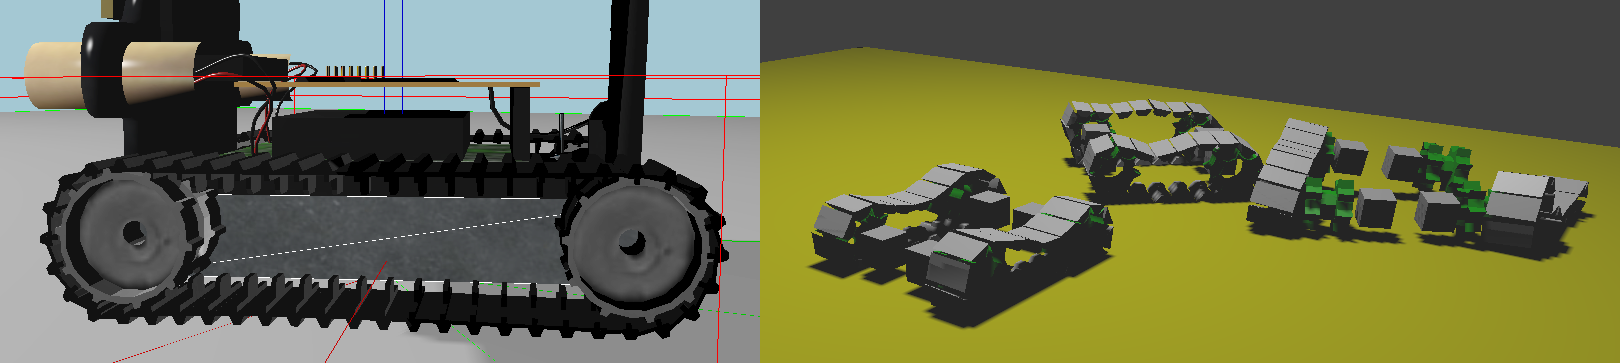
\includegraphics[scale=0.25]{../Figures/Chapter5/treads.png}
\rule{35em}{0.5pt}
\caption[Simulated Treads]{Here you see the to-scale treads modeled after the physical SRV-1 robot on the left and the physics-based rigid-body tracks in motion on the right.}
\label{treads}
\end{figure}

Scale was problematic as the Blender/Bullet physics engine has difficulty with collisions of objects that have a size outside of the assumed range of .05 to 10 meters \cite{website:bulletscale}. Objects smaller than .05 (5cm) Blender/Bullet units, in any given dimension, erratically jitter despite having no force acting upon them. 
%For instance, the wheels on the 3D SRV-1 model which are 2.11cm x 2.45cm x 2.52cm.
As such, since the wheel dimensions of the real SRV-1 are 2.11cm x 2.45cm x 2.52cm, the to-scale 3D model of the SRV-1 was affected by this scale limitation of the physics engine.

To rectify these issues, the physics engine was largely abandoned---in terms of providing the motion model---and was only kept to keep the robots from running through each other and the arena. In its place, a constant linear and angular velocity motion model was developed of which only moves the 3D robot as if it was a single point body. See Figure \ref{blendersimrun} and Figure \ref{sklarplots}. 

\begin{figure}[htbp]
\centering
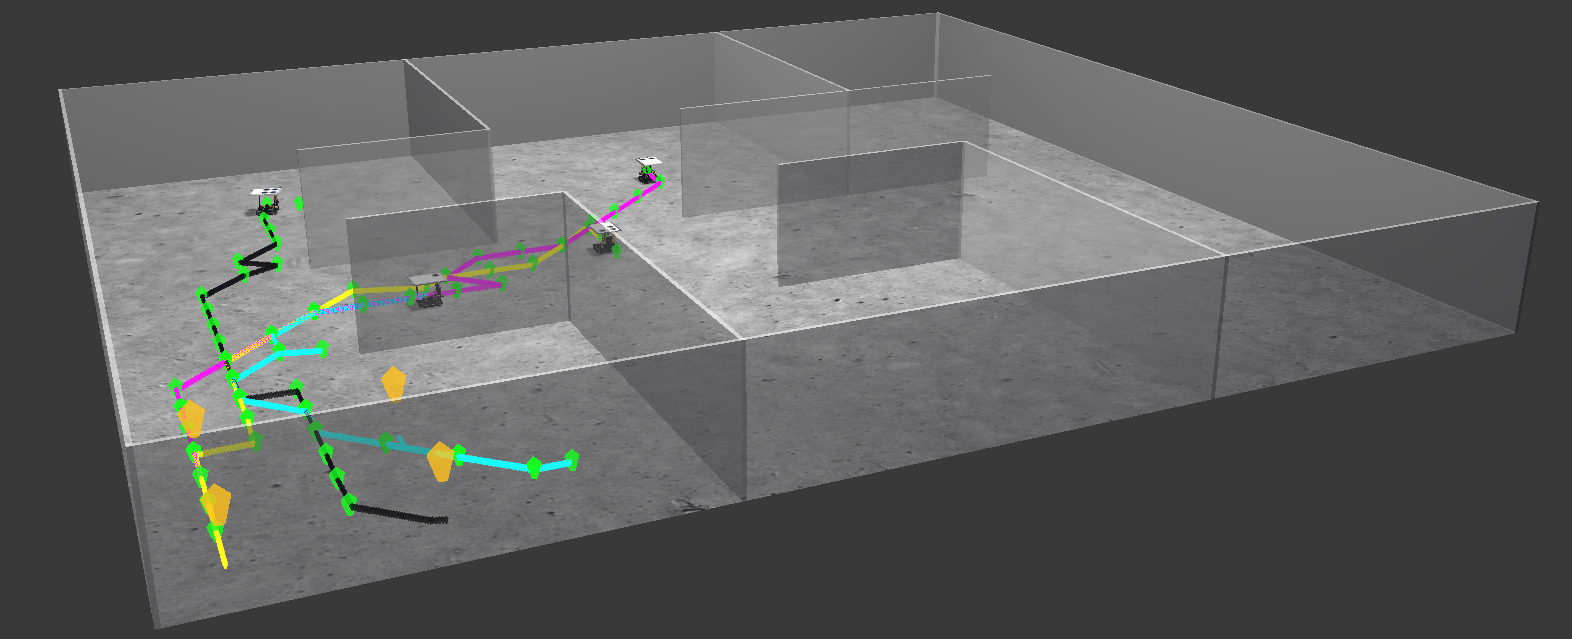
\includegraphics[scale=0.28]{../Figures/Chapter5/const_motion_model.png}
\rule{35em}{0.5pt}
\caption[Constant Velocity Locomotion Model]{Here you see the constant velocity motion model at work in BlenderSim with four robots traversing their respective paths of which consist of way-points scrapped from a previously recorded physical lab experiment.}
\label{blendersimrun}
\end{figure}

\begin{figure}[htbp]
\centering
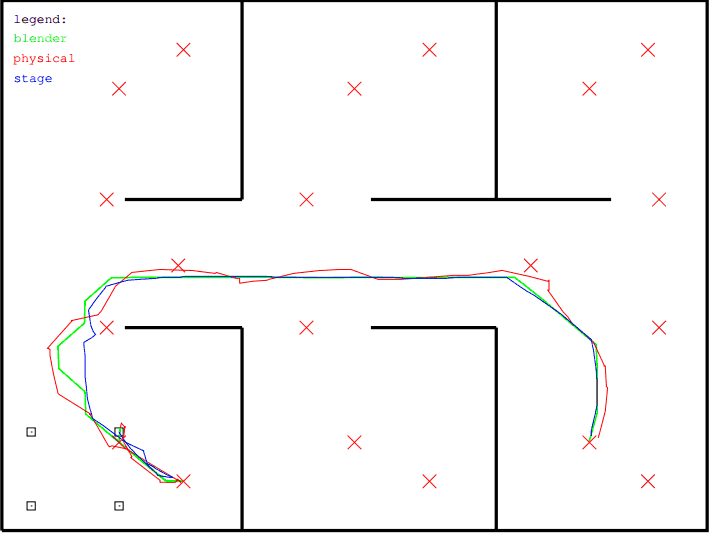
\includegraphics[scale=0.55]{../Figures/Chapter5/const_motion_model_plotted.png}
\rule{35em}{0.5pt}
\caption[Comparative Path Plots]{Here you see the path plots--as plotted by Dr. Elizabeth Sklar--of the BlenderSim robot, the physical robot, and the \textit{Stage} (a 2D robot simulator already in use by HRTeam)\cite{website:stage} robot plotted in comparison.}
\label{sklarplots}
\end{figure}

\section{Implementation}

Stub.

\subsection{Arena}

The arena is a $602cm\times538cm$ enclosure with with a main hallway and six compartments. All walls are physics based and respond accordingly should any robot try to pass through them. See Figure \ref{fig:arena_map}. 

\begin{figure}[htbp]
\centering
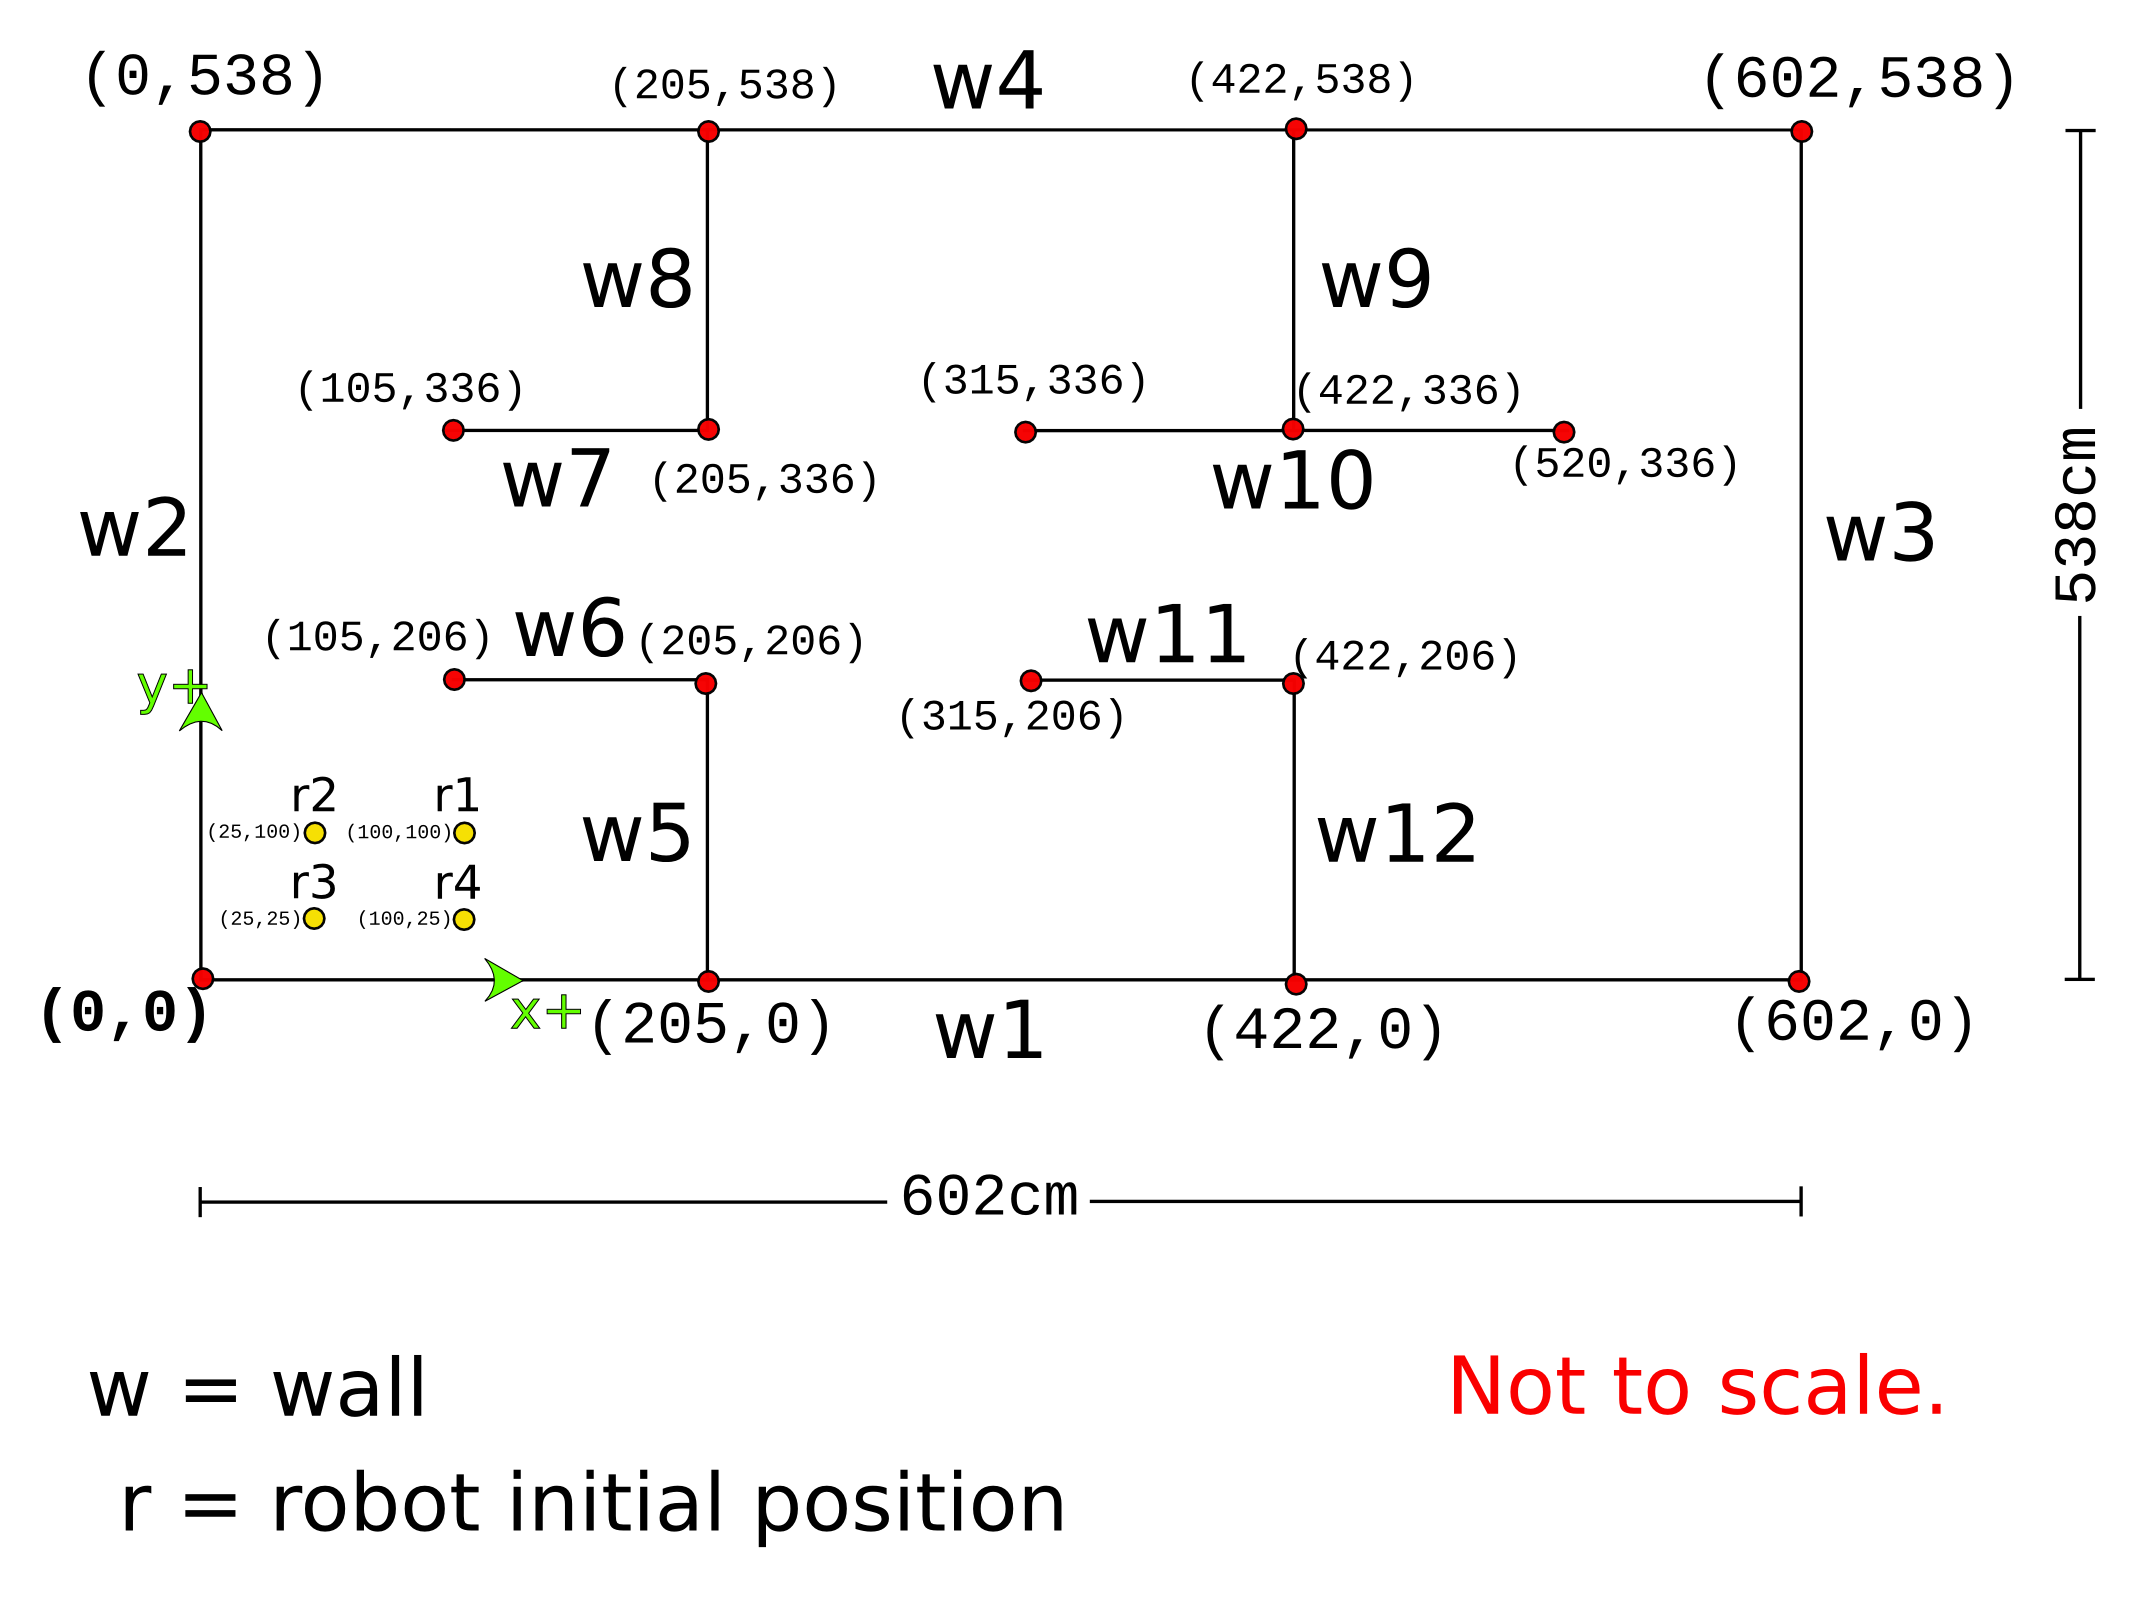
\includegraphics[scale=0.7]{../Figures/Chapter5/map.png}
\rule{35em}{0.5pt}
\caption[BlenderSim Arena]{Here you see the arena map (not to scale) with wall coordinates and robot starting locations.}
\label{fig:arena_map}
\end{figure}

\subsection{Surveyor SRV-1 Blackfin 3D Models}

The 3D model of the Surveyor SRV-1 Blackfin is dimensionally and aesthetically based on the real robot. The extents of the model are $17.64cm\times14.53cm\times14.33cm$ including the braille hat the rests above the body of the robot. The base and the wheels are the only physics based objects on the model with the wheels being connected to the base via a rigid body hinge joint. See Figure \ref{fig:srv1_3d_model}.

\begin{figure}[htbp]
\centering
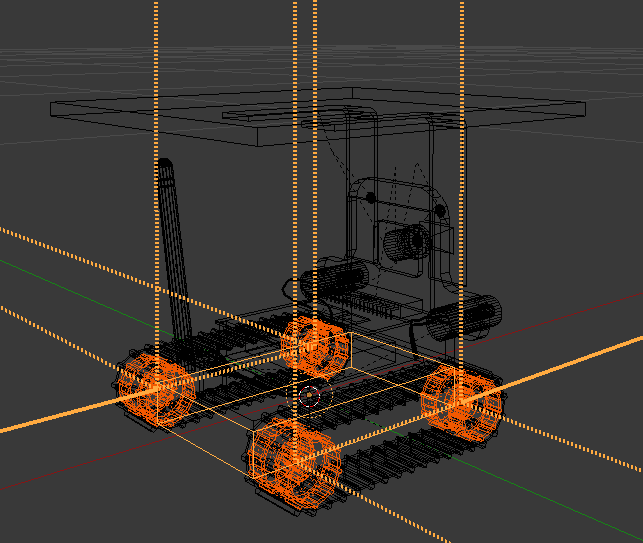
\includegraphics[scale=0.5]{../Figures/Chapter5/srv1.png}
\rule{35em}{0.5pt}
\caption[SRV-1 3D Model]{Here you see the 3D model of the Surveyor SRV-1 Blackfin with the wheels connected to the base via rigid body hinge joints.}
\label{fig:srv1_3d_model}
\end{figure}

\subsection{Robot Servers}

\todo{Change this to reflect when BlenderSim communicates directly with HRTeam.}

The servers are expressed in the simulation as the amber colored \textit{gems} located just above the 3D modeled SRV-1's. See Figure \ref{fig:blendersim_components}. The server logic utilizes the \textit{ServerSocket} Python module. Each of the four servers run in separate threads parented to the Blender process. The four server listen on ports 5001, 5002, 5003 and 5004 respectively. As a connection is made to a client, the server performs a short handshake and begins requesting waypoints from the client. The waypoints are put into a thread safe queue for the robot controller to read from at its leisure. Once the client notifies the server that there are no more waypoints, the server puts \textit{done} in the waypoint queue, sends \textit{done} to the client, shuts down the port, and its thread is terminated.

If the Blender game engine is terminated before the servers receive all of their waypoints, the servers shut down their ports and their threads are terminated. This allows the simulator to be started again fresh (i.e. \textit{$[$Errno 98$]$ Address already in use.} errors) without having to close Blender itself in order to run another simulation.

\subsection{Robot Clients}

\todo{Change this to reflect when BlenderSim communicates directly with HRTeam.}

The four robot clients connect to ports 5001 through 5004 respectively. Utilizing a custom log reader script, the clients read in their respective waypoints from the waypoint logs. Once connected to their respective servers, the clients perform a short handshake and then begin transmitting waypoints as each of their respective servers request them. Once the clients run out of waypoints to transmit, they signal the servers that there are \textit{nomore} waypoints. Once they receive \textit{done} from their respective server, they close the connection and terminate. Out of convenience, a master script runs the four robot clients in four separate asynchronous sub-processes utilizing the \href{http://docs.python.org/2/library/subprocess.html}{\textit{Subproccess}} Python module.

\subsection{Robot Controllers}

\todo{Change this to reflect when BlenderSim communicates directly with HRTeam.}

The robot controllers are expressed in the simulation as the metal box bases of the SRV-1 3D models. See Figure \ref{fig:blendersim_components}. The four robot models are controlled via the logic contained in four robot controllers.
No robot will move while their respective waypoint queues are empty. Once their waypoint queues begin being populated, by their respective servers, the robots will traverse a linear path to each waypoint first by turning to face the waypoint at a constant velocity and then by moving forward towards the waypoint at a constant linear velocity. The velocities were calculated from a historical physical lab experiment log. Once the robots detect \textit{done} in their waypoint queue, they will cease movement indicating that they have traversed the complete \textit{A*} previously-calculated path as read from the historical physical lab experiment master log.

\subsection{Task Points Manager}

\todo{Change this to reflect when BlenderSim communicates directly with HRTeam.}

The task points manager is expressed in the simulation as a large torus located above the 3D modeled arena. Once the Blender game engine is started, it hides itself. See Figure \ref{fig:blendersim_components}. At the start of the simulation, the task points manger reads the task points configurations from the task points configuration directory. Controls include keys \textit{\textbf{a}} through \textit{\textbf{e}} where each key corresponds to the five possible task point configurations. See Figure \ref{fig:task_points}. 

\begin{figure}[htbp]
\centering
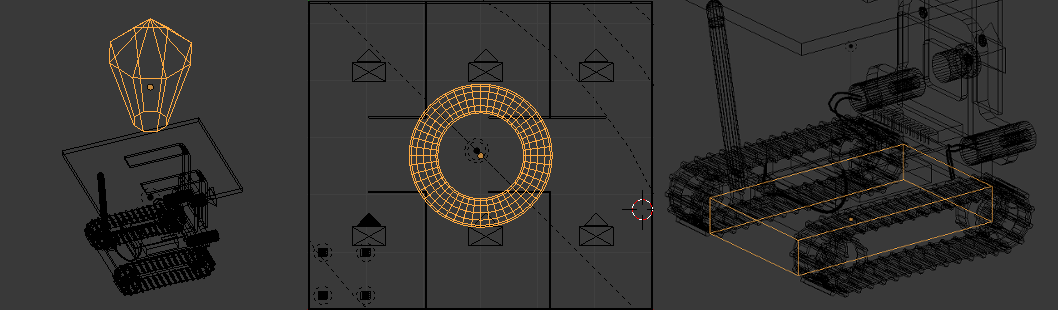
\includegraphics[scale=0.4]{../Figures/Chapter5/parts.png}
\rule{35em}{0.5pt}
\caption[BlenderSim Components]{Here you see from left to right, the server \textit{gem}, the task points manager, and the robot controller manifestations in the simulation.}
\label{fig:blendersim_components}
\end{figure}

\begin{figure}[htbp]
\centering
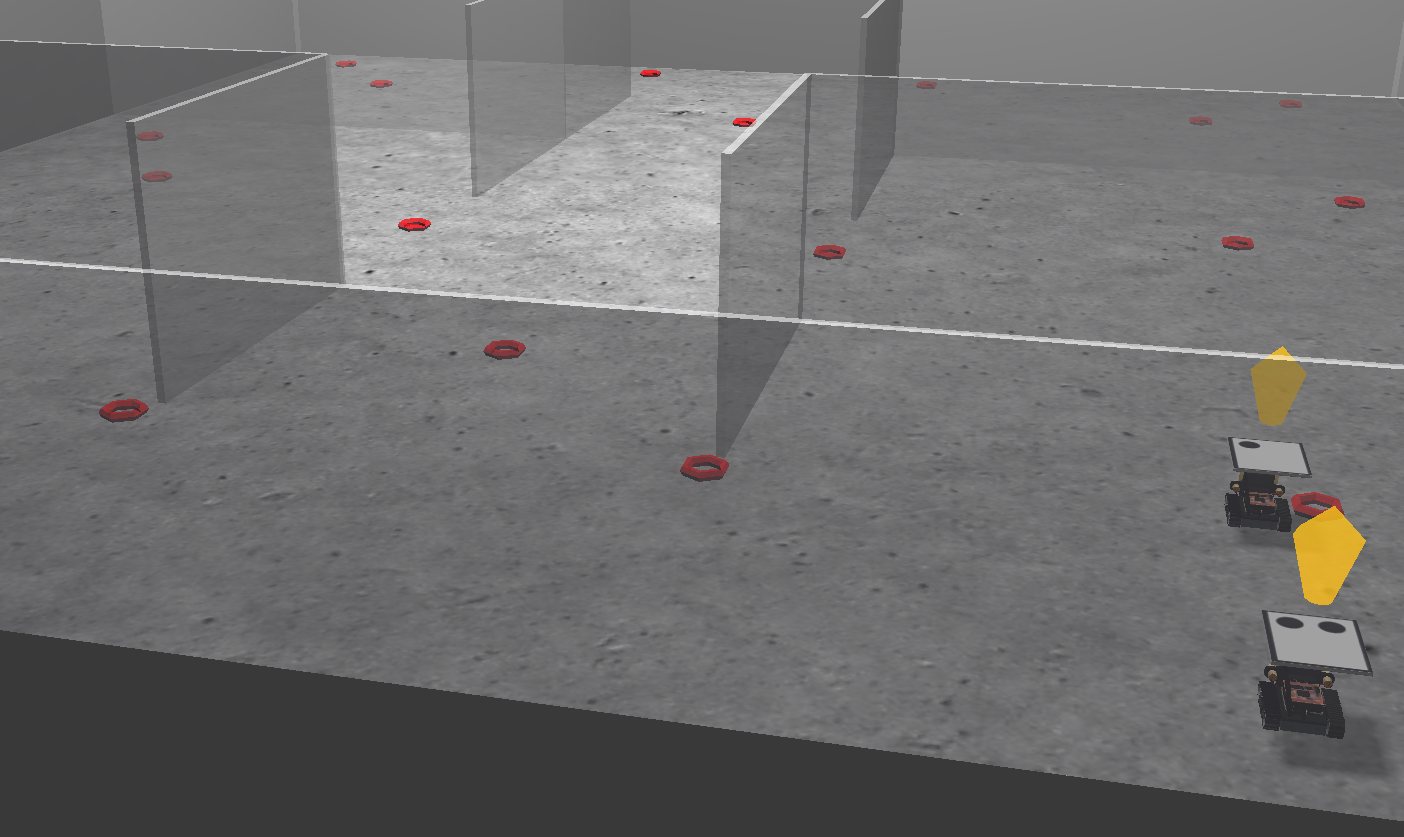
\includegraphics[scale=0.32]{../Figures/Chapter5/taskPoints.png}
\rule{35em}{0.5pt}
\caption[Task Points]{Here you see the red torus task points laid out in the arena.}
\label{fig:task_points}
\end{figure}

\section{Platform}

BlenderSim was run on a 64bit Linux operating system with 32GB of RAM and an Intel Core i7-4770K four core processor running at 3.9GHz.

\section{Experimental Designs}

Stub.

\section{Experimental Results}

Stub.
